\documentclass[notes]{subfiles}
\begin{document}
	\addcontentsline{toc}{section}{12.2 - Vectors}
	\refstepcounter{section}
	\fancyhead[RO,LE]{\bfseries \nameref{cs122}} 
	\fancyhead[LO,RE]{\bfseries \small \currentname}
	\fancyfoot[C]{{}}
	\fancyfoot[RO,LE]{\large \thepage}	%Footer on Right \thepage is pagenumber
	\fancyfoot[LO,RE]{\large Chapter 12.2}
	
\section*{Vectors}\label{cs122}
	\subsection*{Before Class}
	\subsubsection*{Vectors \& Operations}
		\begin{defn}[Vector]
			A \textbf{vector} is a quantity that carries \blank{2} and\\[15pt] \blank{2}.  A \emph{displacement vector} shows how a particle moves from point $A$ to point $B$.  In this case, $A$ is called the \emph{initial point} and $B$ is called the \emph{terminal point}. 
		\end{defn}
		
		\begin{rmk}[Notation]
			For a vector with initial point $A$ and terminal point $B$, we indicate this by writing $\textbf{v} = \overrightarrow{AB}$
		\end{rmk}
		\begin{defn}[Equivalent Vectors]
			Two vectors \textbf{u} and \textbf{v} are \textbf{equal} if they have the same \blank{2}\\[15pt] and \blank{2}.
		\end{defn}
		\begin{defn}[Zero Vector]
			The \textbf{zero vector}, denoted \textbf{0}, is the unique vector with length 0 and no direction.
		\end{defn}
			\newpage
			
		\begin{rmk}[Vector Addition]
			If \textbf{u} and \textbf{v} are vectors positioned so that the \blank{2} of \textbf{v} is the\\[15pt] \blank{2} of \textbf{u}, then the sum $\textbf{u} + \textbf{v}$ whose initial point is the initial point of \textbf{u} and whose terminal point is the terminal point of \textbf{v}.
		\end{rmk}
		\begin{ex}
			Draw the sum of the vectors given below.
		\end{ex}	
			\vs{1}
			
		\begin{defn}[Scalar]
			A \textbf{scalar} is a real number which scales a vector by a certain amount.
		\end{defn}
		\begin{ex}
			Describe the effect of the scalars $-2$, $0$, and $2$ on the vector \textbf{u} drawn below.
		\end{ex}
			\vs{1}
			\newpage
			
		\begin{rmk}[Scalar Multiplication]
			If $c$ is a scalar and \textbf{v} is a vector, then the scalar multiple $c\textbf{v}$ is the vector whose length is \\[15pt] \blank{3} and whose direction is the same as \textbf{v} if $c > 0$ and\\[15pt] opposite to \textbf{v} if $c < 0$.  If $c = 0$ or $\textbf{v} = \textbf{0}$, then $c\textbf{v} = $\blank{1}.
		\end{rmk}
		
	\subsubsection*{Components}
		\begin{defn}[Components]
			If we place the initial point of a vector \textbf{u} at the origin, its terminal point is a coordinate pair $(u_1,u_2)$.  These coordinates are called the \textbf{components} of \textbf{u}, and we write\\[15pt]
					\[\textbf{u} = \hspace{1.5in} \text{or} \hspace{1.5in}\]
		\end{defn}

		\begin{rmk}[Constructing Vectors from Points]
			If the point $A(x_1,y_1,z_1)$ is the initial point of the vector \textbf{u} and $B(x_2,y_2,z_2)$ is the terminal point of \textbf{u}, then we can construct \textbf{u} as\\[15pt]
				\[\textbf{u} = \hspace{2in}\]
		\end{rmk}
		
		\begin{ex}
			Find the vector represented by the directed line segment with initial point $(2,-3,4)$ and terminal point $(-2,1,1)$.
		\end{ex}
			\vs{1}
			
		\begin{ex}
			Find a vector \textbf{a} with representation given by the directed line segment $\overrightarrow{AB}$, if the points are $A(-2,1)$ and $B(1,2)$.
		\end{ex}
			\vs{1}
			\newpage
		
	\subsection*{Pre-Class Activities}
		\begin{ex}
			Use this space to write any questions you might have from the videos.
		\end{ex}
			\vs{.5}
			
		\begin{ex}
			Given the points below, write a vector representation for the directed line segment $\overrightarrow{AB}$.
			\begin{enumerate}[(a)]
				\item $A(-5,-1)$ and $B(-3,3)$
					\vs{1}
					
				\item $A(3,-1)$ and $B(2,3)$
					\vs{1}
					
				\item $A(0,3,1)$ and $B(2,3,-1)$
					\vs{1}
			\end{enumerate}
		\end{ex}
			\newpage
			
	\subsection*{In Class}
	\subsection*{Properties of Vectors}
		\begin{rmk}[Magnitude of a Vector]
			Given a vector $\textbf{a} = \lrangle{a_1,a_2}$, its length is given by\\[15pt]
				\[|\textbf{a}| = \hspace{1.5in}\]
				\\[10pt]
			If $\textbf{a} = \lrangle{a_1,a_2,a_3}$, its length is instead given by\\[15pt]
				\[|\textbf{a}| = \hspace{1.5in}\]
		\end{rmk}
		
		\begin{ex}
			Compute the magnitude of the vectors $\textbf{v} = \lrangle{3,4}$ and $\textbf{u} = \lrangle{2,-2,6}$
		\end{ex}
			\vs{1}
		
		\begin{ex}
			Let $P_1 = (-4,3,1)$ and $P_2 = (-2,5,2)$.
			\begin{enumerate}[(a)]
				\item Let $P_1$ and $P_2$ be the initial and terminal points of a vector $\textbf{v}$.  Find the component form of $\textbf{v}$.
					\vs{1}
					
				\item Find $|\textbf{v}|$.
					\vs{1}
			\end{enumerate}
		\end{ex}	
			\newpage
		
		\begin{rmk}[Algebra of Vectors]
			If $\textbf{a} = \lrangle{a_1,a_2}$, $\textbf{b} = \lrangle{b_1,b_2}$, and $c$ is a scalar, then\\[10pt]
			\begin{itemize}
				\setlength\itemsep{15pt}
				
				\item $\textbf{a} + \textbf{b} = $\blank{2.5}
				\item $\textbf{a} - \textbf{b} = $\blank{2.5}
				\item $c\textbf{a} = $\blank{2.5}
			\end{itemize}\\[10pt]
			The obvious changes are made for three-dimensional vectors.
		\end{rmk}
		\begin{ex}
			Let \textbf{v} be a three-dimensional vector given by $\textbf{v} = \lrangle{v_1,v_2,v_3}$, and let $k\in \R$ be a scalar value.  Show that $|k\textbf{v}| = |k|\,|\textbf{v}|$
		\end{ex}
			\vs{1}
			
		\begin{ex}
			If $\textbf{a} = \lrangle{3,4,0}$ and $\textbf{b} = \lrangle{-1,5,2}$, find $|\textbf{a}|$, $\textbf{a}+\textbf{b}$, $\textbf{a} - \textbf{b}$, $-3\textbf{b}$, and $2\textbf{a} + 4\textbf{b}$.
		\end{ex}	
			\vs{1}
			
		\begin{ex}
			Find $\textbf{a} + \textbf{b}$, $4\textbf{a}+2\textbf{b}$, $|\textbf{a}|$, and $|\textbf{a}-\textbf{b}|$ for the vectors $\textbf{a} = \lrangle{-3,4}$ and $\textbf{b} = \lrangle{9,-1}$.
		\end{ex}
			\vs{1}
			\newpage
		
		\begin{rmk}[Properties of Vectors]
			If \textbf{a}, \textbf{b}, and \textbf{c} are $n-$dimensional vectors, and $c,d$ are scalars, then\\[15pt]
			\begin{itemize}
				\setlength\itemsep{15pt}
				\item $\textbf{a} + \textbf{b} =$ \blank{2}
				\item $\textbf{a} + (\textbf{b} + \textbf{c}) = $\blank{2}
				\item $\textbf{a} + \textbf{0} =$ \blank{1}
				\item $\textbf{a} + \textbf{-a}=$ \blank{1}
				\item $c(\textbf{a} + \textbf{b}) =$ \blank{2}
				\item $(c+d)\textbf{a} = $\blank{2}
				\item $(cd)\textbf{a} =$\blank{1.5}
				\item $1\textbf{a} = $\blank{1}
			\end{itemize}
		\end{rmk}
	
	\subsubsection*{Unit Vectors}
		\begin{ex}
			Let $\textbf{u} =\lrangle{-1,1,2}$
			\begin{enumerate}[(a)]
				\item Find $|\textbf{u}|$
					\vs{1}
					
				\item Find $\left|\dfrac{1}{2}\textbf{u}\right|$
					\vs{1}
				
				\item What happened to the magnitude?  What should we do to \textbf{v} instead to make the magnitude precisely 1?
					\vs{.5}
			\end{enumerate}
		\end{ex}
			\newpage
			
		\begin{defn}[Unit Vector]
			A \textbf{unit vector} is a vector whose magnitude is exactly one.
		\end{defn}
		
		\begin{ex}
			Find the unit vector in the direction of the vector $\lrangle{2,-1,2}$.
		\end{ex}
			\vs{1}
		\begin{rmk}[Finding Unit Vectors]
			Given a vector \textbf{a}, its unit vector $\hat{\mathbf{a}}$ can be found by the formula \blank{2}
		\end{rmk}
		\begin{rmk}[Special Unit Vectors]
			\[\textbf{i} = \lrangle{1,0,0}\hspace{1in}
			\textbf{j} = \lrangle{0,1,0} \hspace{1in}
			\textbf{k} = \lrangle{0,0,1}\]

			These special unit vectors are sometimes called the \textbf{standard basis vectors}.
		\end{rmk}
		
		\begin{ex}
			Express the vector $\lrangle{2,-1,2}$ and its associated unit vector in terms of the standard basis vectors.
		\end{ex}
			\vs{1}
			
		\begin{ex}
			If $\textbf{a} = \textbf{i} +2\textbf{j} - 3\textbf{k}$ and $\textbf{b} = 4\textbf{j} + 8\textbf{k}$, express the vector $2\textbf{a} + 3\textbf{b}$ in terms of the standard basis vectors.
		\end{ex}
			\vs{1}
			\newpage
		
		\begin{ex}
			Find the vector that has the same direction as the vector $\lrangle{1,1,2}$, but with magnitude 14.
		\end{ex}
			\vs{.25}
	\subsubsection*{Applications}		
		\begin{ex}
			A jet, flying due east at 400 mph in still air, encounters a 65-mph tailwind blowing in the direction $40\dc$ north of east.  The airplane holds its compass heading due east, but acquires a new ground speed and direction due to the wind.  What are they?
		\end{ex}
			\vs{1}
			
		\begin{ex}
			A small cart is being pulled along a smooth horizontal floor with a 50-lb force \textbf{F}, making a $60\dc$ angle to the floor.  What is the force moving the cart forward?
		\end{ex}
			\vs{1}
			\newpage
			
		\begin{ex}
			A 100-N weight is suspended by two wires, as shown in the diagram below.  Find the forces $\mathbf{F_1}$ and $\mathbf{F_2}$ acting in both wires.
		\end{ex}
		\begin{flushleft}
			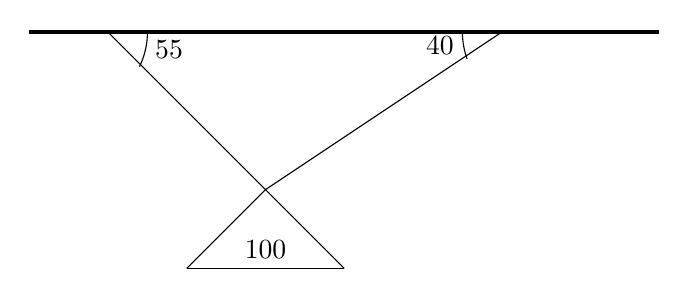
\begin{tikzpicture}
				\draw[very thick] (-4,0)--(4,0);
				\draw (-3,0)--(-1,-2);
				\draw (-1,-2)--(2,0);
				\draw (-2.5,0) arc (0:-26:1) node [midway, right] {$55\dc$};
				\draw (1.5,0) arc(180:200:1) node[midway,left] {$40\dc$};
				\draw (-2,-3)--(-1,-2)--(0,-3);
				\draw (-2,-3)--(0,-3) node[midway, above] {100};
			\end{tikzpicture}
		\end{flushleft}

			\newpage
	\subsection*{After Class Activities}
		\begin{ex}
			Find $\textbf{a} + \textbf{b}$, $4\textbf{a} + 2\textbf{b}$, $|\textbf{a}|$, and $|\textbf{a} - \textbf{b}|$ for the following vectors.
			\begin{enumerate}[(a)]
				\item $\textbf{a} = 5\textbf{i} + 3\textbf{j}$, $\textbf{b} = -\textbf{i} - 2\textbf{j}$
					\vs{2}
					
				\item $\textbf{a} = \lrangle{8,1,-4}$, $\textbf{b} = \lrangle{5,-2,1}$
					\vs{2}
			\end{enumerate}
		\end{ex}
		
		\begin{ex}
			Find the vector in the same direction as $\lrangle{6,2,-3}$, but with length 4.
		\end{ex}
			\vs{1}
			
		\begin{ex}
			If \textbf{v} lies in the first quadrant and makes an angle of $\dfrac{\pi}{3}$ with the positive $x-$axis, and has a magnitude of 5, find \textbf{v} in component form.
		\end{ex}
			\vs{1}
			
		\begin{ex}
			A child pulls a sled through the snow on a level path with a force of 50 N, exerted at an angle of $38\dc$ above the horizontal.  Find the horizontal and vertical components of the force.
		\end{ex}
			\vs{1}
			\newpage
			
		\begin{ex}
			A woman walks due west on the deck of a ship at 3 mi/h.  The ship is moving north at a speed of 22 mi/h.  Find the speed and direction of the woman relative to the surface of the water.
		\end{ex}
			\vs{1}
			
		\begin{ex}
			Three forces act on an object.  Two of the forces are at an angle of $100\dc$ to each other and have magnitudes 25 N and 12 N. The third is perpendicular to the plane of these two forces and has magnitude 4 N.  Calculate the magnitude of the force that would exactly counterbalance these three forces.
		\end{ex}
			\vs{1}
		
			
\clearpage
\end{document}
